\documentclass{beamer}
\usepackage[utf8]{inputenc}
\usepackage{hyperref}
\usepackage{amsmath,amsfonts,amsthm,bm}
\usepackage{color}
\usepackage{graphicx} % Allows including images
\usepackage{tikz}
\usepackage{mhchem}
\usepackage{pgfplots}
\usepackage{multirow}

\hypersetup{
    colorlinks=true,
    linkcolor=red,
    filecolor=magenta,      
    urlcolor=red,
}

\DeclareMathOperator*{\argmax}{argmax}
\DeclareMathOperator*{\argmin}{argmin}
\let \vec \mathbf

\mode<presentation> {
    \usetheme{CambridgeUS}
    %\setbeamertemplate{footline} % To remove the footer line in all slides uncomment this line
    \setbeamertemplate{footline}[page number] % To replace the footer line in all slides with a simple slide count uncomment this line
    \setbeamertemplate{navigation symbols}{} % To remove the navigation symbols from the bottom of all slides uncomment this line
}


\title[NANO281 Review]{NANO281 Review}

\author{Shyue Ping Ong}
\institute[UCSD]{University of California, San Diego\\
\medskip
}
\date{NANO281} % Date, can be changed to a custom date

\begin{document}


\begin{frame}
    \titlepage % Print the title page as the first slide
\end{frame}


\begin{frame}{Overview}
    \tableofcontents
\end{frame}


\section{Review}


\begin{frame}{Preliminaries}
    \begin{itemize}
        \item In this class, we have provided a broad survey of data science techniques as they are applied to materials science problems.
        \item In doing so, we have opted for breadth rather than depth, and eschewed most of the mathematical derivations that is typical in data science classes.
        \item In this final lecture, I want to do an overview of the coverage to reinforce the lessons learnt.
        \item The structure of this overview is deliberately different from the sequence in which we have done the entire class. Now that you have the details in your mind, this lecture provides a high-level overview of key takeaways and guiding principles.
    \end{itemize}
\end{frame}


\begin{frame}{Why Data Science?}
    \begin{itemize}
        \item Materials data is exploding in quantity and quality.
        \begin{itemize}
            \item High-throughput/combinatorial experiments.
            \item High-throughput first principles computations.
        \end{itemize}
        \item Types of problems that can most benefit from data science:
        \begin{itemize}
            \item Things that are still too difficult to perform experiments on or compute.
            \item Relationships that are beyond our understanding (at the present moment). 
        \end{itemize}
    \end{itemize}
\end{frame}


\begin{frame}{ML flowchart}
\begin{figure}
    \centering
    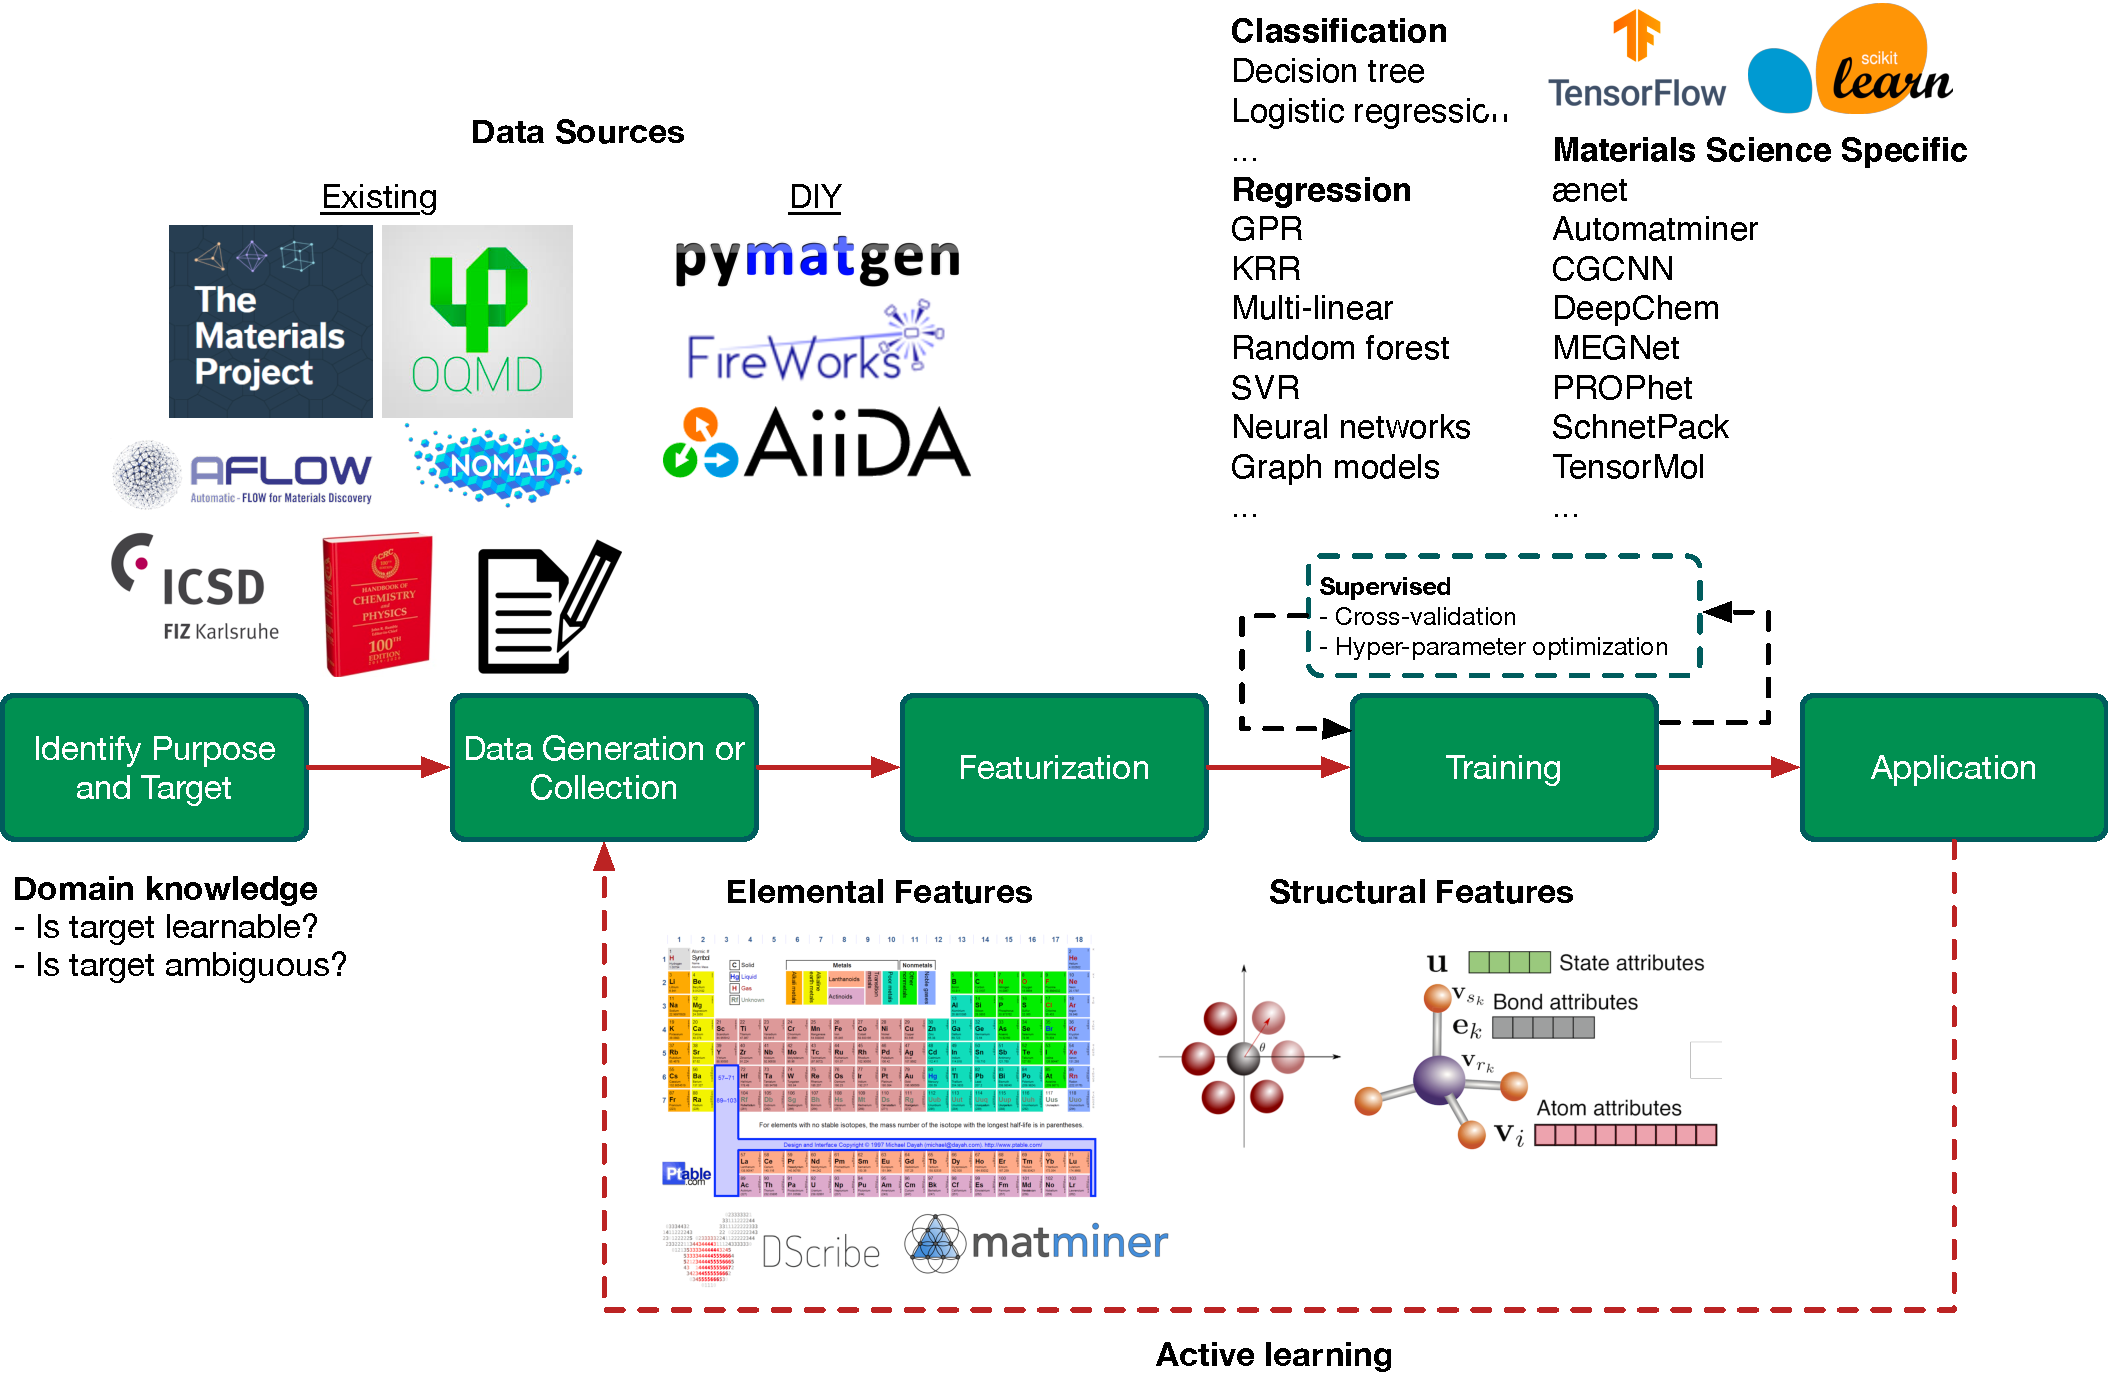
\includegraphics[width=\textwidth]{figures/ml_flowchart.pdf}
\end{figure}
\end{frame}


\begin{frame}{Data and Featurization}
    \begin{itemize}
        \item Data generation, collection and wrangling is typically the most time-consuming portion of the whole process.
        \item Sources: Experimental (\href{http://icsd.fiz-karlsruhe.de/icsd/}{ICSD}, \href{http://paulingfile.com/}{Pauling file}, literature, ...), Computational (\href{http://www.materialsproject.org}{Materials Project}, \href{http://oqmd.org/}{OQMD}, \href{http://aflowlib.org/}{AFLOW}, \href{https://nomad-coe.eu/}{NOMAD}, ...).
        \item Quality and quantity remains a big issue in materials science.
        \item Featurization - typically the choice that affects model performance the most
        \begin{itemize}
            \item Composition-based features (e.g., electronegativity, atomic radii, etc.): intuitively simple, readily available, but clearly cannot capture structural differences.
            \item Structure-based features (including graphs): much greater complexity, typically must obey symmetries of system to be effective.
        \end{itemize}
    \end{itemize}
\end{frame}


\begin{frame}{Model fitting}
    \begin{itemize}
        \item All model fittings follow the same basic principle - minimizing of some \textit{loss function}, $L(\theta; y_i, \vec{x_i})$ either analytically or by numerical procedures (e.g., gradient descent).
    \end{itemize}
        \begin{table}[h]
        \scriptsize
            \centering
            \begin{tabular}{l|l|l}
                Task & Loss function & Equation \\
                \hline
             \multirow{2}{*}{Regression} & Mean squared error & $
        \sum_{i=1}^N (y_i - f(x_i))^2$\\
        & Mean absolute error & $
        \sum_{i=1}^N |y_i - f(x_i)|$\\
               \hline \multirow{4}{*}{Classification} & Missclassification rate & $I(\mathrm{sign}(f) \neq y)$\\
               & Exponential loss & $e^{-yf(x)}$\\
                 & Binomial/multinomial &
        $-\sum_{k=1}^K I(y=G_k)f_k(x) + \log \left(\sum_{l=1}^K e^{f_l(x)}\right)$\\
        & Binomial deviance & $\log(1 + e^{-2yf})$
            \end{tabular}
        \end{table}
\end{frame}


\begin{frame}{Model assessment and selection}
    \begin{itemize}
        \item Model performance is related to its performance on \textit{independent test data}.
        \begin{itemize}
            \item Training error: $L$ over training set.
            \item Test error: $L$ over independent test set.
        \end{itemize}
        \item Model complexity increases as the number of parameters increases. 
        \item Training errors \textbf{always} decrease with increasing model complexity.
        \item Test errors are high when model complexity is too low (underfitting) or too high (overfitting).
    \end{itemize}
    \begin{figure}
        \centering
        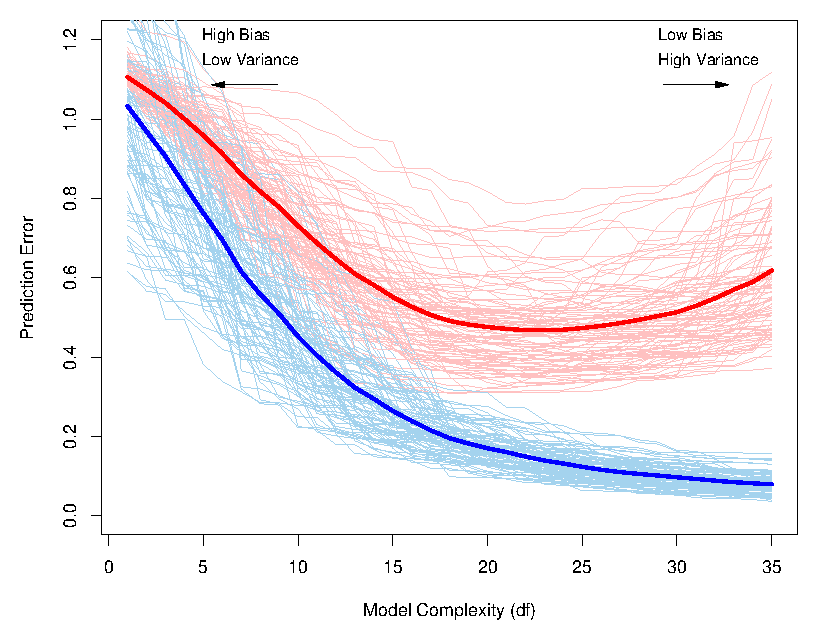
\includegraphics[width=0.4\textwidth]{figures/fig7-1.pdf}
    \end{figure}
\end{frame} 


\begin{frame}{Training, validation and test data}
    \begin{itemize}
        \item Model selection: estimating the performance of different models in order to choose the best one.
        \item Model assessment: having chosen a final model, estimating its prediction error (generalization error) on new data.
        \begin{itemize}
            \item Training set: For training the model.
            \item Validation set: For estimating prediction error to select the model.
            \item Test set: For assessing the generalization error of the final model. This should not be used in fitting the model.
        \end{itemize}
        \item Typical training:validation:test split is 50:25:25 or 80:10:10, or in very data-poor situations, maybe even 90:5:5.
    \end{itemize}
\end{frame}


\begin{frame}{$K$-fold cross validation (CV)}
    \begin{itemize}
        \item Simplest and most widely used approach for model validation.
        \item Data set is split into $K$ buckets (usually by random).
        \item Typical values of $K$ is 5 or 10. $K = N$ is known as ``leave-one-out'' CV.
        \begin{table}
        \begin{tabular}{|p{1.7cm}|p{1.7cm}|p{1.7cm}|p{1.7cm}|p{1.7cm}|}
            \hline
            \Large{Train} & \Large{Train} & \textcolor{red}{\Large{Validate}} & \Large{Train} & \Large{Train}\\
            \hline
        \end{tabular}
        \end{table}
        \item CV score is computed on the validate data set after training on the train data:
        \begin{equation*}
                CV(\hat{f}^{-k(i)},\alpha) = \frac{1}{N_{k(i)}}\sum_{i=1}^{N_{k(i)}} L(y_i, \hat{f}^{-k(i)}(x_i,\alpha))
        \end{equation*}
        \item assuming the $k^{th}$ data bucket has $N_{k(i)}$ data points and $\hat{f}^{-k(i)}$ refers to the model fitted with the $k^{th}$ data left out.
    \end{itemize}
\end{frame}


\begin{frame}{Regularization}
    \begin{itemize}
        \item Often, one starts from a model that is more complex first, and then reduce model complexity.
        \item Reducing model complexity decreases risk of overfitting (improve generalizability).
        \begin{itemize}
            \item Shrink coefficients or weights, sometimes to zero.
            \item Subset selection / tree pruning.
        \end{itemize}
        \item General approach is to add a \textit{penalty term} to loss functions that penalizes overcomplex models, e.g., sum of squares or absolute value of coefficients (e.g., MLR) or weights (NNs), tree size (decision trees), etc. Controlled by some parameter to be specified by model developer that determines size of penalty.
        \item Bias-variance trade-off:
        \begin{equation*}
            \mathrm{MSE} = \mathrm{var}(\hat{\theta}) + [E(\hat{\theta}) - \theta]^2
        \end{equation*}
    \end{itemize}
\end{frame}


\begin{frame}{Types of ML models}
    \begin{itemize}
        \item Supervised learning
        \begin{itemize}
            \item Linear (MLR, Ridge, Lasso, Linear/Quadratic Discriminant)
            \item Local/Kernel methods (kNN, kernel density estimation, Gaussian mixture models)
            \item Trees (CART, Adaboost, Gradient Boosting, Random Forest)
            \item Neural networks
        \end{itemize}
        \item Unsupervised learning
        \begin{itemize}
            \item Principal Component Analysis
            \item K-means
            \item DBSCAN
        \end{itemize}
        \item And many others that have not been covered (e.g., support vector machines, graph-based models, etc.)
    \end{itemize}
\end{frame}


\section{Final Lab}


\begin{frame}{Final Lab}
    \begin{itemize}
        \item 
    \end{itemize}
\end{frame}


\begin{frame}{Bibliography}
    \bibliographystyle{unsrt}
    \bibliography{refs}
\end{frame}


\begin{frame}
    \Huge{\centerline{The End}}
\end{frame}

\end{document}

